\subsection[prof]{Profiling}

\begin{frame}[fragile]
  \frametitle{Profiling}
  \begin{block}{Conceptually}
    \begin{itemize}
      \item Take a measurement of a performance aspect of a program
      \begin{itemize}
        \item Where in my code is most of the time spent?
        \item Is my program compute or memory bound?
        \item Does my program make good use of the cache?
        \item Is my program using all cores most of the time?
        \item How often are threads blocked and why?
        \item Which API calls are made and in which order?
        \item ...
      \end{itemize}
      \item The goal is to find performance bottlenecks
      \item Usually done on a compiled program, not on source code
    \end{itemize}
  \end{block}
\end{frame}

\begin{frame}[fragile]
  \frametitle{\mintinline{bash}{perf} -- Performance analysis tools for Linux}
  \setlength{\leftmargini}{0pt}
    \begin{itemize}
      \item Powerful command line profiling tool for Linux
      \item Not portable, the source code is part of the Linux kernel itself
      \item Much lower overhead compared with \mintinline{bash}{valgrind}
      \item In order to profile your code, make sure to compile with
            \texttt{CXXFLAGS="-O2 -g -fno-omit-frame-pointer"}
      \item Counting and sampling
        \begin{itemize}
          \item Counting -- count occurrences of a given event (e.g.\ cache misses)
          \item Time-based sampling -- sample the stack at regular time intervals
          \item Event-based sampling -- take samples when event counter overflows
          \item Instruction-based sampling -- sample instructions and precisely count events they create
        \end{itemize}
      \item Static and dynamic tracing
        \begin{itemize}
          \item Static -- pre-defined tracepoints in software (e.g.\ scheduling events)
          \item Dynamic -- tracepoints created dynamically with \mintinline{bash}{perf probe}
        \end{itemize}
    \end{itemize}
\end{frame}

\begin{frame}[fragile]
  \frametitle{\mintinline{bash}{perf} commands}
  { \scriptsize
    \begin{block}{}
      \begin{minted}{shell-session}
$ perf
 usage: perf [--version] [--help] [OPTIONS] COMMAND [ARGS]
 The most commonly used perf commands are:
   annotate        Read perf.data and display annotated code
   c2c             Shared Data C2C/HITM Analyzer.
   config          Get and set variables in a configuration file.
   diff            Read perf.data and display the differential profile
   evlist          List the event names in a perf.data file
   list            List all symbolic event types
   mem             Profile memory accesses
   record          Run a command and record its profile into perf.data
   report          Read perf.data and display the profile
   sched           Tool to trace/measure scheduler properties (latencies)
   script          Read perf.data and display trace output
   stat            Run command and gather performance counter statistics
   top             System profiling tool.
   version         display the version of perf binary
   probe           Define new dynamic tracepoints
   trace           strace inspired tool
 See 'perf help COMMAND' for more information on a specific command.
      \end{minted}
    \end{block}
  }
\end{frame}

\begin{frame}[fragile]
  \frametitle{Listing events with \mintinline{bash}{perf list}}
  { \scriptsize
    \begin{block}{}
      \begin{minted}{shell-session}
$ # List main hardware events
$ perf list hw

List of pre-defined events (to be used in -e):

  branch-instructions OR branches                    [Hardware event]
  branch-misses                                      [Hardware event]
  cache-misses                                       [Hardware event]
  cache-references                                   [Hardware event]
  cpu-cycles OR cycles                               [Hardware event]
  instructions                                       [Hardware event]

$ # List main software/cache events
$ perf list sw
$ perf list cache

$ # List all pre-defined metrics
$ perf list metric

$ # List all currently known events:
$ perf list
      \end{minted}
    \end{block}
  }
\end{frame}

\begin{frame}[fragile]
  \frametitle{Counting events with \mintinline{bash}{perf stat}}
  { \scriptsize
    \begin{block}{}
      \begin{minted}{shell-session}
$ # Standard CPU counter statistics for the specified command:
$ perf stat <command>

$ # Detailed CPU counter statistics for the specified command:
$ perf stat -d <command>
$ perf stat -dd <command>

$ # Top-down microarchitecture analysis for the entire system, for 10s:
$ perf stat -a --topdown -- sleep 10

$ # L1 cache hit rate reported every 1000 ms for the specified command:
$ perf stat -e L1-dcache-loads,L1-dcache-load-misses -I 1000 <command>

$ # Instruction per cycle and Instruction-level parallelism, for command:
$ perf stat -M IPC,ILP -- <command>

$ # Measure GFLOPs system-wide, until Ctrl-C is used to stop:
$ perf stat -M GFLOPs

$ # Measure cycles and instructions 10 times, report results with stddev:
$ perf stat -e cycles,instructions -r 10 -- <command>
      \end{minted}
    \end{block}
  }
\end{frame}


\begin{frame}[fragile]
  \frametitle{Recording profiling information with \mintinline{bash}{perf record}}
  { \scriptsize
    \begin{block}{}
      \begin{minted}{shell-session}
$ # Sample on-CPU functions for the specified command, at 100 Hertz:
$ perf record -F 100 -- <command>

$ # Sample CPU stack traces (via frame pointers), at 100 Hertz, for 10s:
$ perf record -F 100 -g -- sleep 10

$ # Sample stack traces for PID using DWARF to unwind stacks, for 10s:
$ perf record -p <PID> --call-graph=dwarf -- sleep 10

$ # Precise on-CPU user stack traces (no skid) using PEBS (Intel CPUs):
$ perf record -g -e cycles:up -- <command>

$ # Sample CPU stack traces using Instruction-based sampling (AMD CPUs):
$ # (Note that you need to use system-wide sampling for IBS on AMD CPUs)
$ perf record -a -g -e cycles:pp -- <command>

$ # Sample CPU stack traces once every 10k L1 data cache misses, for 5s:
$ perf record -a -g -e L1-dcache-load-misses -c 10000 -- sleep 5

$ # Sample CPUs at 100 Hertz, and show top addresses and symbols, live:
$ perf top -F 100
      \end{minted}
    \end{block}
  }
\end{frame}

\begin{frame}[fragile]
  \frametitle{Reporting and annotating source code with \mintinline{bash}{perf}}
  { \scriptsize
    \begin{block}{}
      \begin{minted}{shell-session}
$ # Standard reporting of perf.data in text UI interface:
$ perf report

$ # Report by self-time (excluding time spent in callees):
$ perf report --no-children

$ # Report per source line of code (needs debugging info to work):
$ perf report --no-children -s srcline

$ # Single inverted (caller-based) call-graph per binary:
$ perf report --inverted -s comm

$ # Text-based report per library, without call graph:
$ perf report --stdio -g none -s dso

$ # Hierarchical report for functions taking at least 1% of runtime:
$ perf report --stdio -g none --hierarchy --percent-limit 1

$ # Disassemble and annotate a symbol (instructions with percentages):
$ # (Needs debugging information available to show source code as well)
$ perf annotate <symbol>
      \end{minted}
    \end{block}
  }
\end{frame}

\begin{frame}[fragile]
  \frametitle{Further information on \mintinline{bash}{perf}}
  \begin{itemize}
    \item Official documentation in the Linux repository at
    \href{https://git.kernel.org/pub/scm/linux/kernel/git/torvalds/linux.git/tree/tools/perf/Documentation}
         {linux/tools/perf/Documentation}
    \item Perf Wiki at \url{https://perf.wiki.kernel.org/}
    \item Linux \mintinline{bash}{perf} examples by Brendan Gregg
          \url{https://www.brendangregg.com/linuxperf.html}
    \item Scripts to visualize profiles as flamegraphs
          \url{https://github.com/brendangregg/FlameGraph}
    \item HSF Tools \& Packaging Working Group talk on Indico\\
          \href{https://indico.cern.ch/event/974382/}
          {Linux Systems Performance: Tracing, Profiling \& Visualization}
  \end{itemize}
\end{frame}

\begin{frame}[fragile]
  \frametitle{Intel VTune Profiler}
  \centering
  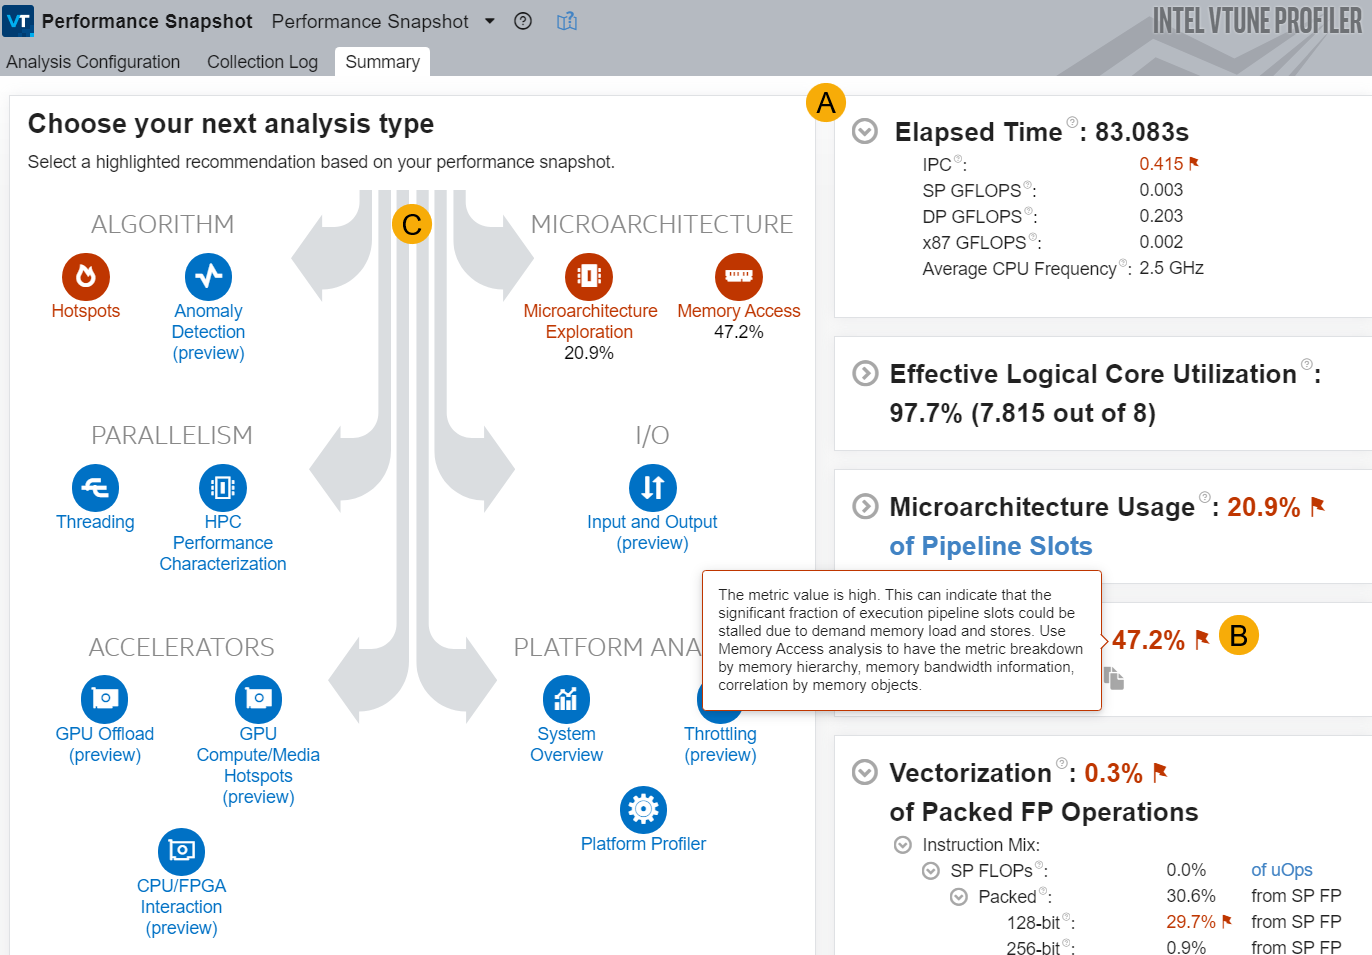
\includegraphics[width=0.75\textwidth]{tools/vtune.png}
  \begin{itemize}
    \item Very powerful GUI-based profiler for Intel CPUs and GPUs
    \item Now free to use with
      \href{https://www.intel.com/content/www/us/en/developer/tools/oneapi/toolkits.html}{Intel oneAPI Base Toolkit} or
      \href{https://www.intel.com/content/www/us/en/developer/tools/oneapi/vtune-profiler.html}{standalone}
    \item See the \href{https://www.intel.com/content/www/us/en/develop/documentation/vtune-help/}
                       {official online documentation} for more information
  \end{itemize}
\end{frame}
